\documentclass[10pt]{report}
\usepackage{graphicx}
\begin{document}
\qquad \qquad \textbf{DEVENDRA KUMAR JANGIR} \\
------------------------------------------------------------------------------------------------------\\
11-A,Vivek Nagar \quad\quad\qquad\qquad\qquad\qquad\qquad Contact:\mbox{9454190392} \\ 
Behind District Stadium \quad\qquad\qquad\qquad\qquad Email: \texttt{devendraj592@gmail.com} \\
Jhunjhunu(Rajasthan)   \\
PIN-333001    \\
\begin{figure}[h]
\qquad\qquad\qquad\qquad\qquad\qquad\qquad\qquad\qquad\qquad\qquad\qquad
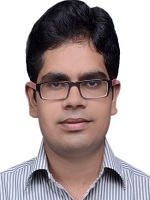
\includegraphics{Dev.jpg}
\end{figure}  \\ \\
\textbf{CAREER OBJECTIVE:} To work in a challenging environment demanding all my skills and efforts to explore and adapt myself in different fields and realise my potential where i get the opportunity for continuous learning. \\ \\
\textbf{EDUCATION:}  \\
    \begin{tabular}{|c|p{2cm}|p{2.5cm}|c|c|}
    \hline
    Degree & College/School & Board/University & Passing year & Pass percentage  \\
    \hline
    High School & Keshav adarsh vidya mandir & RBSE & 2007 & 87.3 \\
    \hline
    Intermediate & Kendriya vidyalaya & CBSE & 2009 & 87.4  \\
    \hline
    B.tech(ECE) & JKIAPT & Allahabad University & 2015 & 72   \\
    \hline
    \end{tabular}   \\ \\ \\
\textbf{PROJECTS:}
    \begin{enumerate}
    \item \textbf{Seed sowing bot:-} It is a microcontroller based automated device which is used to detect holes and then dropping the defined number of seeds in it accordingly. 
    \item \textbf{Transistor polarity checker(mini project):-} The aim of this project was to design a hardware which could be used to check transistor polarity that is whether it is npn or pnp type.
    \item \textbf{Home automation system:-} The aim of this project was to design a hardware using microcontrollers which could be used to control any electrical device [220 v , 4 amp]
    \item \textbf{A Pedometer circuit:-} A pedometer or distance counter is a device usually portable and electronic or electro mechnanical,that counts each step of a person takes by detecting the motion of the person’s feet
    \item \textbf{Care taker bot:-} The aim of this project was to design a caretaker bot which fulfils patients requests, as
    directed by a host-pc which process images taken via a webcam over an arena resembling a hospital floor
    \item \textbf{PC Controlled two wheel balance bot:-} The aim of this project was to make a two wheel balance bot which can
    balance itself without any extra support and control its motion through PC
    \end{enumerate}
    \qquad\\
 \textbf{TRAINING AND INTERNSHIPS:} 
    \begin{itemize}
    \item Basic robotics workshop by BISD labs
    \item Embedded And Robotoics Advanced at IIIT Allahabad from HPES
    \item Eyantra summer internship at IIT Bombay
    \end{itemize}
    \quad\\ 
\textbf{RESEARCH PUBLICATIONS:}  
\qquad\qquad NIL    \\ \\
\textbf{TECHNICAL SKILLS:} 
    \begin{itemize}
    \item C and Embedded C
    \item Python and opencv
    \item Embedded System and Robotics,Communication systems
    \item Firebird,PCB express,AVR studio
    \end{itemize}
    \qquad\\  
\textbf{SOFTSKILS:}
    \begin{enumerate}
    \item Diligent
    \item Quick learner
    \item Adaptable
    \item Team worker and patient
    \end{enumerate}   
    \qquad\\
\textbf{EXTRA-CURRICULAR ACTIVITIES:}
    \begin{itemize}
    \item Participated in many SINGING events
    \item District level winner of singing competition at school level. 
    \item Was one of the Anchors in AVIRBHAV'14(Annual Fest)
    \item Member of organising committee of AVIRBHAV'14
    \item Participated in Flash mob-a dancing event under AVIRBHAV'14
    \end{itemize}  
    \qquad\\
\textbf{Co-CURRICULAR ACTIVITIES:}
    \begin{enumerate}
    \item Won first prize under E-yantra robotics competition 2015
    \item Secured seventh position under E-yantra robotics competition 2014
    \item Got appreciation award from \textbf{HEWLETT PACKARD} during summer training
    \item Participated in many circuit designing competition
    \item Brand ambassdor of HPES(Allahabad region) for one year(2012-13) 
    \end{enumerate}   
    \qquad\\
\textbf{HOBBIES:}
   \begin{itemize}
   \item Singing
   \item Listening to music
   \item Diary writing
   \item Solving sudoku
   \item Internet Surfing
   \end{itemize}       
   \qquad\\
\textbf{PERSONAL DETAILS:}
   \begin{itemize}
   \item Father's Name :- Murari Lal Jangir
   \item Mother's Name :- Shimala Devi
   \item Sex :- Male
   \item Nationality :- Indian
   \item Marital Status :- Unmarried
   \end{itemize}
   \qquad\\ 
\textbf{DECLARATION:}
\\ \\ I hereby declare that the particular given herein are true to my knowledge and belief. \\ \\ \\
\textbf{DATE: } \qquad\qquad\qquad\qquad\qquad\qquad\qquad\qquad\qquad\qquad\qquad\qquad\qquad Signature



\end{document}